%% 美赛模板:正文部分

\documentclass[12pt]{article}  % 官方要求字号不小于 12 号,此处选择 12 号字体

% 本模板不需要填写年份,以当前电脑时间自动生成
% 请在以下的方括号中填写队伍控制号
\usepackage[2116733]{easymcm}  % 载入 EasyMCM 模板文件
\problem{F}  % 请在此处填写题号
\usepackage{mathptmx}  % 这是 Times 字体,中规中矩 
\usepackage{mathpazo}  % 这是 COMAP 官方杂志采用的更好看的 Palatino 字体,可替代以上的 mathptmx 宏包
\usepackage{tabularx}

\title{Model Construction and Evaluation in Higher Education}  % 标题

% 如需要修改题头(默认为 MCM/ICM),请使用以下命令(此处修改为 MCM)
%\renewcommand{\contest}{MCM}

% 文档开始
\begin{document}

% 此处填写摘要内容
\begin{abstract}

Since the second half of the 20th century, due to the widespread needs of the society for all kinds of high-level talents, higher education has achieved unprecedented development and has affected all aspects of human society. We selected 9 important indicators of the higher education system in 5 representative countries (the United States, France, Japan, Brazil and India), and established a set of models to evaluate the health of a country’s higher education system and predict its sustainability.
\vspace{5mm}

In the first part, we constructed an index set to evaluate the health of a country's higher education system. Then, we collected and screened 9 main indicators into the indicator set, and standardized them. After that, we used the principal component analysis method (PCA) to reduce the dimensionality of the selected indicators to obtain three main components, which simplified the difficulty of establishing the model.
\vspace{5mm}

In the second part, we applied the BP neural network model, and trained it through standard data set , and took the United States and India as the best and worst scales to construct a national higher education health evaluation model. In this process, we discovered many shortcomings of the BP neural network model, and applied particle swarm algorithm to improve the model. The final optimized results are: US LV5, France LV3, Japan LV3, Brazil LV2 and India LV1.
\vspace{5mm}

In the third part, we use the gray forecast model. We took the indicators of these 5 countries in the past 5 years as samples, and predict the trend of the indicators in the next 3 years. Then brought the results into the evaluation model to get the higher education system of 5 countries Sustainability ratings: US LV5, France LV4, Japan LV3, Brazil LV2 and India LV1.
\vspace{5mm}

In the fourth part, taking Japan as an example, we proposed a policy for increasing enrollment rate and brought it into our model for verification. The results show that this policy can increase Japan's higher education health and sustainability ratings by one level after three years. At the same time, we analyzed the impact of the policy and admitted that it is very difficult to implement this policy.
\vspace{5mm}

At the end of the paper, we also analyzed the advantages and disadvantages of our model, and proposed some possible improved algorithms, such as adding momentum terms, improving the learning rate, and combining intelligent algorithms. In addition, we have also made a reasonable promotion of the model so that it can be applied to a wider range of fields.
\vspace{8mm}

\textbf{Key words}: PCA, BP neural network model, PSO, Grey prediction model


    % 美赛论文中无需注明关键字。若您一定要使用,
    % 请将以下两行的注释号 '%' 去除,以使其生效
    

\end{abstract}

\maketitle  % 生成 Summary Sheet
\tableofcontents  % 生成目录


% 正文开始
\section{Introduction}
\subsection{Problem Background}
Since the second half of the 20th century, due to the widespread needs of the society for all kinds of high-level talents, higher education has achieved unprecedented development and has affected all aspects of human society. From a global perspective, the penetration rate of higher education is steadily increasing. Statistics from the World Bank show that the global higher education enrollment rate has increased from 9.7\% in 1970 to 38.8\% in 2019, especially after the 21st century, this data has grown rapidly at an annual rate of 1\%. In 2000, Chinese scholar Pan Maoyuan pointed out that the transition from the elite stage to the popularization stage of higher education is not only an increase in quantity, but also a “qualitative” change, including the expansion of educational functions, the diversification of training objectives and educational models, curriculum settings, and A series of changes in teaching methods and methods, admission requirements, management methods, and the relationship between higher education and society. In the process of gradual development and popularization of higher education, these speculations have also been verified. Then, how to reasonably evaluate the development level of higher education in a country or region, and how to show whether the status quo of higher education in a country is perfect? Clarifying the answers to these questions plays an important role in the improvement and improvement of the global higher education evaluation mechanism.



\subsection{Restatement of the Tasks}


\begin{itemize}
   
   

 \item Part I: Develop and verify a set of models that can evaluate the health of the higher education system in any country; apply this set of models to several countries, and then select one of the countries where the higher education system has room for improvement based on the analysis; In this regard, this article will adopt principal component analysis and BP neural network to build a model, and apply it to several representative countries.

\item Part II: Propose an achievable and reasonable vision for the selected country’s system to support a healthy and sustainable higher education system; use the model to measure the health of the current system, and propose for the selected country , Healthy and sustainable system.

\item Part III: Propose targeted policies and implementation timelines to support the migration from the current state to your proposed state. Use your model to shape and evaluate the effectiveness of your policies.

\item Part IV: Considering that change is difficult in reality, discuss the impact of the plan implemented during the transition period and in the final state on the real world (for example, students, teachers, communities, countries); we will integrate the country’s society In practice, compare theoretical predictions with actual applications, and analyze the impact of the plan.

\end{itemize}

\subsection{Glossary}
\begin{itemize}

\item Higher Education: The optional final stage of formal learning that occurs after completing the required secondary education level. In this article, higher education is the core of our analysis, and all questions are raised and answered inseparable from the discussion of higher education.

\item Sustainable system: A system that maintains its effectiveness over time. This article will use models to ensure the sustainability of our proposed policies.

\item System health: Measure an organization or system around a common vision, effectively implement the vision, and update its ability through innovation and creative thinking. This article will evaluate the health of the original system based on the constructed model.

\item Higher education system: the organizational structure composed of higher education institutions (colleges, universities, etc.) and the personnel and infrastructure required to educate students above secondary. In this article, we will evaluate the higher education systems of different countries and give corresponding development suggestions for one of them.




\end{itemize}



\subsection{Past work}
Due to the different national conditions of countries in the world, there is no unified higher education evaluation standard in the world, but there are still some scientific evaluation systems that have been widely recognized. For example, Quacquarelli Symonds (QS) uses academic reputation (40\%), employer reputation (10\%), teacher-student ratio (20\%), citation rate per faculty member (20\%), international teacher ratio (5\%), and international students The ratio (5\%) is used to evaluate the educational level of the university in six aspects. In addition, international research scholars generally believe that the evaluation criteria should be positioned reasonably, enriched continuously, and keep pace with the times.


\section{Preparation of the Models}
\subsection{Assumptions}
\begin{enumerate}[\bfseries 1.]

\item Assume that the relevant data collected in various countries are true and reliable.

\item Assume that only the nine factors mentioned in this paper represent all the factors that may affect higher education

\item Assume that only the five countries mentioned in the paper represent all the countries to be analysed.

\item In practice, colleges and universities produce a small amount of extreme data because of complex situations. Assuming that the appearance of extreme data is negligible compared with conventional data, it will not affect the research section.

\end{enumerate}

\subsection{Notations}
The primary notations used in this paper are listed in Table \ref{tb:notation}.

% 三线表示例
\begin{table}[!htbp]
\begin{center}
\caption{Notations}
\begin{tabular}{cl}
	\toprule
	\multicolumn{1}{m{3cm}}{\centering Symbol}
	&\multicolumn{1}{m{8cm}}{\centering Definition}\\
	\midrule
	
	$r\left(X_{i},X_{j}\right)$&Correlation coefficient between  $X_{i}$ \ and \  $X_{j}$\\
	
	$\operatorname{Cov}\left(X_{i}, X_{j}\right)$&Covariance of  \ $X_{i}$ \ and \ $X_{j}$\\
	
	
	$F_{i}$
    $\left(\mathrm{i}=1, 2, \cdots, m\right)$&The score of factor\ $F_{i}$\ on\ variable\ $X_{p}$\\
	
	$\alpha_{i}$
    $\left(\mathrm{i}=1, 2, \cdots, m\right)$&Contribution rate of factor $F_{i}$\\
	
	$z_{k}$&Hidden layer node output\\


	$y_{i}$&The output of the output layer node\\
	
	$\eta$ &Learning rate\\

	$\Delta v_{ik}$ &Adjusted hidden layer neuron weights\\
	
	$A1$ &The past strength of higher education\\
	$A2$ &The current strength of higher education\\
	$A3$ &The future strength of higher education\\
	\bottomrule

	
	
\end{tabular}\label{tb:notation}
\end{center}
\end{table}









\section{The Models}
\subsection{Overview}


\begin{figure}[h!]
\centering
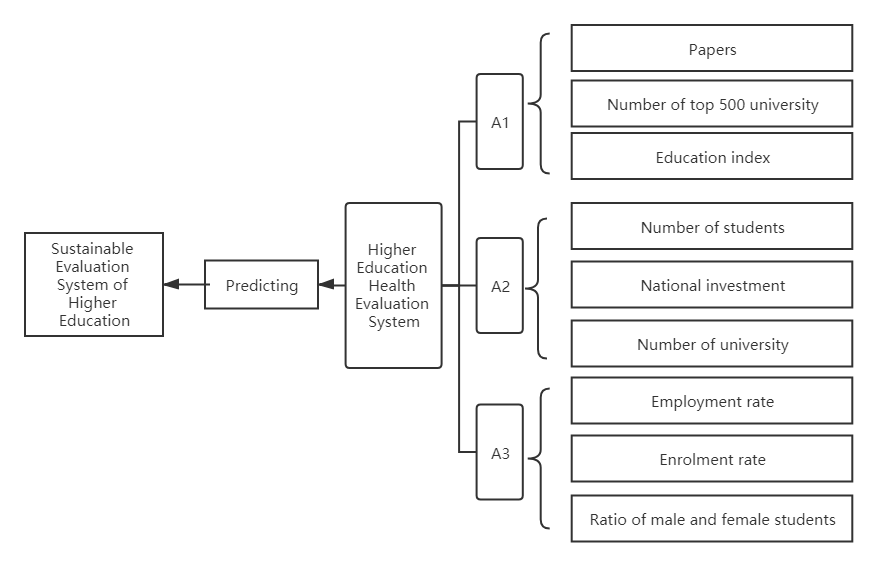
\includegraphics[scale=0.5]{biao2.png}
\caption{Overview}
\label{fig:GVT}
\end{figure}


It can be seen from reading the questions that this question can be divided into two parts. The first part is an evaluation question, which requires us to establish a model to evaluate the health of higher education systems in various countries; the second part is a prediction question, which requires us to base on the predicted results Make suggestions and predict effects. Therefore, this article will describe the model building process in two parts.

\subsection{Health Evaluation Index}
\subsubsection{Screening indicators}

There are many indicators to measure the level of higher education in a country. Therefore, it is necessary to screen the indicators. We initially selected 12 indicators through Wikipedia, the World Bank and other websites. They are:

\begin{enumerate}[\bfseries 1.]
    \item The number of papers 
    \item The number of top 500 universities 
    \item The number of Nobel Prize winners
    \item The number of Fields Medal winners
    \item The education index
    \item The Number of students
    \item The ratio of male to female students.
    \item Scientific research input-output ratio
    \item Employment rate
    \item The number of education funds invested by the state
    \item The number of total universities
    \item The enrollment rate
\end{enumerate}

Taking into account the weakness of some countries with low education levels in indicators such as awards, for the accuracy of the model, we have eliminated some indicators and finally retained 9 indicators to more accurately measure a country’s education from the past to the future The health of the system.


\subsubsection{Processing of sample data}

When performing multivariate statistical analysis, the data collected are of different dimensions, and there are differences in orders of magnitude or measurement units between them, so the various variables are not comprehensive. If the indicators are used directly, the results will be greatly affected by the magnitude of some indicators, or the calculation results will not have practical significance due to the inconsistent measurement units [6].

Therefore, the standardized processing of data is very necessary. The standardization of data is also called dimensionless processing. In this way, the influence of dimensions and orders of magnitude among various indicators can be eliminated, so that the data can be processed objectively and accurately.

Next, the data is normalized, and the linear function is used to convert the original data linearization method to the range of [0, 1]. The normalization formula is as follows:
\begin{equation}\label{eq:eq1}
X_{\text {norm }}=\frac{X-X_{\min }}{X_{\max }-X_{\min }}\end{equation}

Among them, $X_{\text {norm }}$ is the normalized data, X is the original data, and $X_{\text {max }}$, $X_{\text {min }}$ are the maximum and minimum values of the original data set.

This method achieves equal scaling of the original data.

\subsubsection{Use principal component analysis to reduce the dimensionality of indicators}

The above processing of sample data is still not enough. This is because if you directly analyze the selected 9 indicator data, it will be affected by noise and extreme data, and at the same time, the processing speed will be affected by too much data. Therefore, it is necessary to reduce the dimensionality of the selected indicators. Since each indicator has nothing to do with the year [7], the principal component analysis is done directly on the five-year data of five countries and a total of 25 samples.

\textbf{Applicability test of principal component analysis:}

Let $r\left(X_{i}, X_{j}\right)$ be the correlation coefficient between index $X_{i}$ and index $X_{j}$, then

\begin{equation}\label{eq:eq2}r\left(X_{i}, X_{j}\right)=\frac{\operatorname{Cov}\left(X_{i}, X_{j}\right)}{\sqrt{\operatorname{Var}\left[X_{i}\right] \operatorname{Var}\left[X_{j}\right]}}\end{equation}

Among them, $Cov\left(X_{i}, X_{j}\right)$ is the covariance of $X_{i}$ and $X_{j}$, $\operatorname{Var}\left[X_{i}\right]$ is the variance of $X_{i}$, and $\operatorname{Var}\left[X_{j}\right]$ is the variance of $X_{j}$.

We can judge whether the principal component analysis method is feasible according to the size of the correlation coefficients among all index variables. If most of  $r\left(X_{i}, X_{j}\right)$  is greater than or equal to 0.3, it indicates that the principal component analysis method is initially feasible.

\textbf{"KMO" ("Kaiser-Meyer-Olkin") test:}

The statistics of this test are used to compare the simple correlation and partial correlation coefficients between variables.

The KMO value is between 0-1, and the closer it is to 1, it indicates that the sum of squares of simple correlation coefficients between all variables is much larger than the sum of squares of partial correlation coefficients, and the more suitable for principal component analysis.

Among them, Kaiser gave a KMO inspection standard:

KMO > 0.9, very suitable;

0.8< KMO < 0.9, suitable; 

0.7 < KMO < 0.8, general; 

0.6 < KMO<0.7, not suitable; 

KMO < 0.6, not suitable.


The calculation shows that the correlation coefficients between all index variables are greater than 0.3, and the "KMO" test value is 0.671, and principal component analysis can be used.

\textbf{Extraction of principal components:}

Take the data of the United States as an example, use spss to extract the principal components of the data, and the results are shown in the figure:


\begin{figure}[h!]
\centering
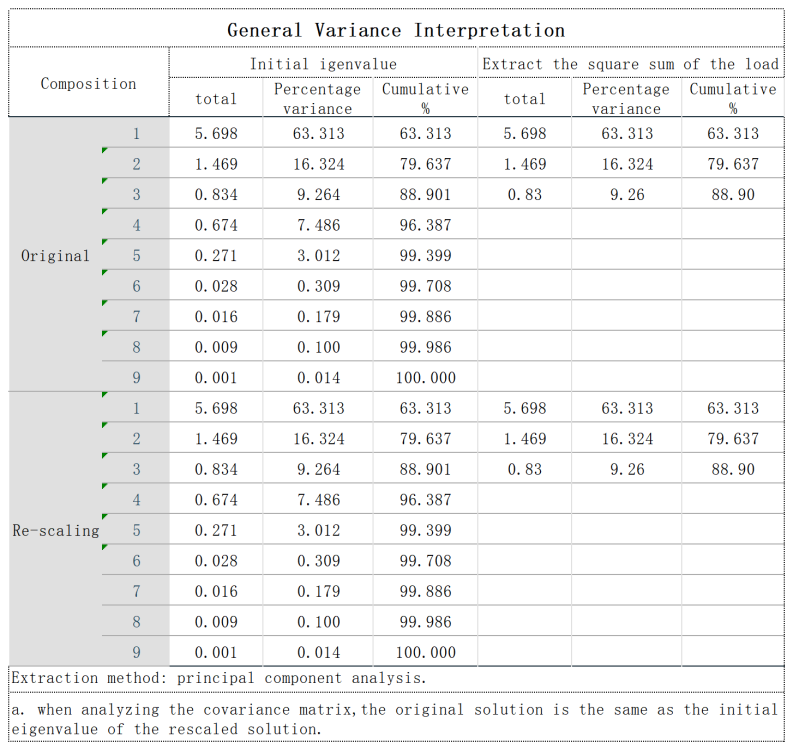
\includegraphics[scale=0.7]{biao1.png}
\caption{General Variance Interpretation}
\label{fig:GVT}
\end{figure}

The total variance explained by the invariant principal component analysis shows that the cumulative contribution rate of the three principal components can reach 88.9\%, which can reflect the original variables to a large extent, thus achieving the reduction of data dimensionality.

For convenience and intuition, we rename these three variables as: A1-the past strength of higher education, A2-the current strength of higher education, and A3-the future strength of higher education.

Perform the above operations in sequence for the remaining countries to obtain all the data of these countries after dimensionality reduction.

\textbf{Calculated score:}

According to the factor score coefficient and standardized data, the score of each component is obtained. The formula is:
\begin{equation}\label{eq:heat3}F_{i}=\beta_{i 1} X_{1}+\beta_{i 2} X_{2}+\cdots+\beta_{i n} X_{n}\end{equation}

$F_{i}$is the score of factor $F_{i}$ on variable $X_{p}$.

The expression of the comprehensive score of the principal component is:

\begin{equation}\label{eq:heat3}\left\{\begin{array}{l}
\mathrm{A} 1=0.563^{*} \mathrm{~F}_{1}-0.420^{*} \mathrm{~F}_{2}-0.187^{*} \mathrm{~F}_{3} \\
\mathrm{~A} 2=0.977^{*} \mathrm{~F}_{4}-0.966^{*} \mathrm{~F}_{5}-0.580^{*} \mathrm{~F}_{6} \\
\mathrm{~A} 3=-0.990^{*} \mathrm{~F}_{7}+0.991^{*} \mathrm{~F}_{8}+0.992 * \mathrm{~F}_{9}
\end{array}\right.\end{equation}

$F_{i}$
$\left(\mathrm{i}=1, 2, \cdots, m\right)$ is the score of each component, $\alpha_{i}$
$\left(\mathrm{i}=1, 2, \cdots, m\right)$ is the contribution rate of each component.

In summary, through the principal component analysis method, the original 9 indicators are reduced into 3 new indicators.

\subsubsection{Result of the problem}

In the above stage, 9 indicators for evaluating the national education system were initially screened through data collection, and the indicators were reduced to 3 new indicators through standardized processing and principal component analysis, which laid the foundation for the establishment of the subsequent evaluation model.

\subsection{Model 1: The Health Evaluation  Model }
\subsubsection{General idea}
In order to establish a national higher education health evaluation model, we use the three indicators obtained above to establish an evaluation system through the BP neural network, and use standard data for training. When selecting the evaluation criteria, we divided the fitness into 5 levels, the United States as the highest level 5, and India as the lowest level 1 for training to get the final result.


\subsubsection{Overview of BP neural network}
The BP (Back Propagation) network was proposed by a team of scientists led by Rinehart and McClelland in 1986. It is a multi-layer feedforward network trained by the error back propagation algorithm and is currently one of the most widely used neural network models. The BP network can learn and store a large number of input-output pattern mapping relationships without revealing the mathematical equations describing this mapping relationship in advance. Its learning rule is to use the steepest descent method to continuously adjust the weights and thresholds of the network through backpropagation to minimize the sum of squared errors of the network. The topological structure of the BP neural network model includes an input layer (input), a hidden layer (hide layer) and an output layer (output layer), as shown in the following figure:  

\begin{figure}[h!]
\centering
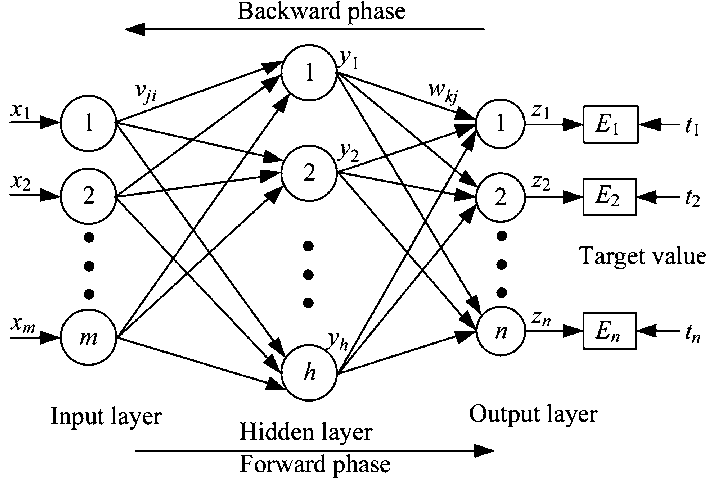
\includegraphics[scale=0.9]{figure1.png}
\caption{BP neural network}
\label{fig:bp1}
\end{figure}

 The BP algorithm consists of two processes: the forward calculation (forward propagation) of the data stream and the backward propagation of the error signal. In forward propagation, the propagation direction is input layer→hidden layer→output layer, and the state of each layer of neurons only affects the next layer of neurons. If the desired output is not available in the output layer, turn to the back propagation flow of the error signal. Through the alternation of these two processes, the error function gradient descent strategy is implemented in the weight vector space, and a group of weight vectors are searched dynamically iteratively to make the network error function reach the minimum value, thereby completing the information extraction and memory process.

\begin{figure}[h!]
\centering
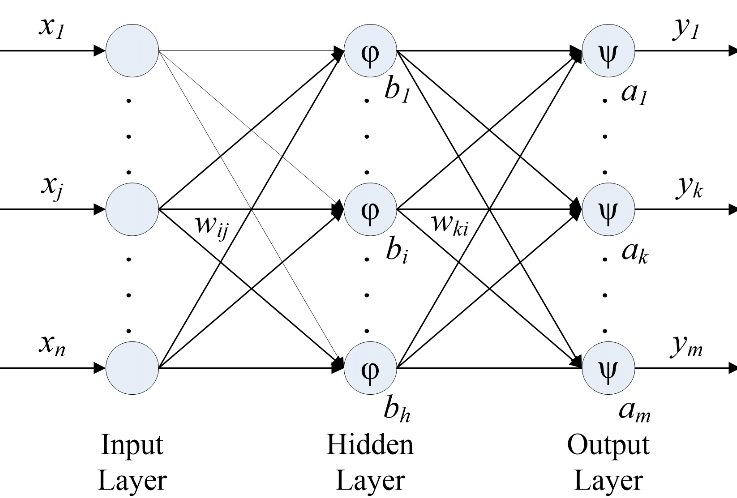
\includegraphics[scale=0.5]{f2.png}
\caption{three-layer BP neural network}
\label{fig:bp2}
\end{figure}

Suppose the input layer of the BP network has n nodes, the hidden layer has q nodes, and the output layer has m nodes. The weight between the input layer and the hidden layer is $v_{k i}$ , and the weight between the hidden layer and the output layer is  $w_{j k}$ .

The transfer function of the hidden layer is f1, and the transfer function of the output layer is f2, then the output of the hidden layer node is (write the threshold into the sum term):

\begin{equation}\label{eq:heat4}z_{k}=f_{1}\left(\sum_{i=0}^{n} v_{k i} x_{i}\right)   
 \ \ \ \mathrm{k}=1, 2, \cdots, q\end{equation}

The output of the output layer node is:

\begin{equation}\label{eq:heat5}y_{j}=f_{2}\left(\sum_{k=0}^{q} w_{j k} z_{k}\right)
 \ \ \ \mathrm{j}=1, 2, \cdots,m
\end{equation}

So far, the BP network has completed the approximate mapping of the n-dimensional space vector to the m-dimensional space.

\textbf{Define error function}

Enter $p$ learning samples, denoted by $x^{1},x^{2},\cdots,x^{p}$. After the  $p$-th sample is input to the network, the output  $y_{j}^{p}  \ \ \ 
\left(\mathrm{j}=1, 2, \cdots,m .\right)$ is obtained.

Using the square error function, the error $E_{p}$ of the $p$-th sample is obtained:

\begin{equation}\label{eq:heat6}
\ E_{p}=\frac{1}{2} \sum_{j=1}^{m}\left(t_{j}^{p}-y_{j}^{p}\right)^{2}\end{equation}

Where: \ $t_{j}^{p}$ is the expected output.

For $p$ samples, the global error is:


\begin{equation}\label{eq:heat7}E=\frac{1}{2} \sum_{y=1}^{P} \sum_{j=1}^{m}\left(t_{j}^{p}-y_{j}^{p}\right)=\sum_{y=1}^{P} E_{y}\end{equation}

\textbf{ Changes in output layer weights:}

The cumulative error BP algorithm is used to adjust $w_{j k}$ to make the global error $E$ smaller, that is


\begin{equation}\label{eq:heat8}\Delta w_{j k}=-\eta \frac{\partial E}{\partial w_{j k}}=-\eta \frac{\partial}{\partial w_{j k}}\left(\sum_{y=1}^{p} E_{y}\right)=\sum_{y=1}^{p}\left(-\eta \frac{\partial E_{y}}{\partial w_{j k}}\right)\end{equation}

Where: $\eta$ is the learning rate.

Define the error signal as:

\begin{equation}\label{eq:heat8}\delta_{y i}=-\frac{\partial E_{y}}{\partial S_{j}}=-\frac{\partial E_{y}}{\partial y_{j}} \cdot \frac{\partial y_{j}}{\partial S_{j}}\end{equation}

The first item:

\begin{equation}\label{eq:heat9}\frac{\partial E_{y}}{\partial y_{j}}=\frac{\partial}{\partial y_{j}}\left[\frac{1}{2} \sum_{j=1}^{m}\left(t_{j}^{y}-y_{j}^{y}\right)^{2}\right]=-\sum_{j=1}^{m}\left(t_{j}^{y}-y_{j}^{y}\right)\end{equation}

The second item:

\begin{equation}\label{eq:heat10}\frac{\partial y_{j}}{\partial S_{j}}=f_{2}^{\prime}\left(S_{j}\right)\end{equation}

Is the partial differential of the transfer function of the output layer.
Then:


\begin{equation}\label{eq:heat11}\delta_{y i}=\sum_{j=1}^{m}\left(t_{j}^{y}-y_{j}^{y}\right) f_{2}^{\prime}\left(S_{j}\right)\end{equation}

From the chain theorem:

\begin{equation}\label{eq:heat12}\frac{\partial E_{y}}{\partial w_{j k}}=\frac{\partial E_{y}}{\partial S_{j}} \cdot \frac{\partial S_{j}}{\partial w_{j k}}=-\delta_{y^{\prime}} z_{k}=-\sum_{j=1}^{m}\left(t_{j}^{y}-y_{j}^{y}\right) f_{2}^{\prime}\left(S_{j}\right) \cdot z_{k}\end{equation}

Then the weight adjustment formula of each neuron in the output layer is:

\begin{equation}\label{eq:heat13}\Delta w_{j k}=\sum_{y=1}^{P} \sum_{j=1}^{m} \eta\left(t_{j}^{y}-y_{j}^{y}\right) f_{2}^{t}\left(S_{j}\right) z_{k}\end{equation}

Changes in hidden layer weights:

\begin{equation}\label{eq:heat14}\Delta v_{k i}=-\eta \frac{\partial E}{\partial v_{k i}}=-\eta \frac{\partial}{\partial v_{k i}}\left(\sum_{y=1}^{p} E_{y}\right)=\sum_{p=1}^{p}\left(-\eta \frac{\partial E_{p}}{\partial v_{k i}}\right)\end{equation}

Define the error signal as:

\begin{equation}\label{eq:heat15}\delta_{z k}=-\frac{\partial E_{y}}{\partial S_{k}}=-\frac{\partial E_{y}}{\partial z_{x}} \cdot \frac{\partial z_{k}}{\partial S_{k}}\end{equation}

The first item:

\begin{equation}\label{eq:heat15}\frac{\partial E_{y}}{\partial z_{k}}=\frac{\partial}{\partial z_{k}}\left[\frac{1}{2} \sum_{j=1}^{m}\left(t_{j}^{y}-y_{j}^{y}\right)^{2}\right]=-\sum_{j=1}^{m}\left(t_{j}^{y}-y_{j}^{y}\right) \frac{\partial y_{j}}{\partial z_{k}}\end{equation}

From the chain theorem:

\begin{equation}\label{eq:heat15}\frac{\partial y_{j}}{\partial z_{k}}=\frac{\partial y_{j}}{\partial S_{j}} \cdot \frac{\partial S_{j}}{\partial z_{k}}=f_{2}^{\prime}\left(S_{j}\right) w_{j k}\end{equation}

The second item:
\begin{equation}\label{eq:heat15}\frac{\partial z_{k}}{\partial S_{k}}=f_{1}^{\prime}\left(S_{k}\right)\end{equation}

Is the partial differential of the hidden layer transfer function.
Thus:

\begin{equation}\label{eq:heat15}\delta_{zk}=\sum_{j=1}^{m}\left(t_{j}^{y}-y_{j}^{p}\right) f_{2}^{\prime}\left(S_{j}\right) w_{j k} f_{1}^{\prime}\left(S_{k}\right)\end{equation}

From the chain theorem:

\begin{equation}\label{eq:heat15}\frac{\partial E_{y}}{\partial v_{k i}}=\frac{\partial E_{y}}{\partial S_{k}} \cdot \frac{\partial S_{k}}{\partial v_{k i}}=-\delta_{z k} x_{i}=-\sum_{j=1}^{m}\left(t_{j}^{y}-y_{j}^{y}\right) f_{2}^{\prime}\left(S_{j}\right) w_{j k} f_{1}^{\prime}\left(S_{k}\right) \cdot x_{i}\end{equation}

Thus, the weight adjustment formula of the neurons in the hidden layer is:

\begin{equation}\label{eq:heat15}\Delta v_{k i}=\sum_{y=1}^{p} \sum_{j=1}^{m} \eta\left(t_{j}^{y}-y_{j}^{y}\right) f_{2}^{\prime}\left(S_{j}\right) w_{j k} f_{1}^{\prime}\left(S_{k}\right) x_{i}\end{equation}

\subsubsection{Model establishment}

The modeling of speech feature signal classification algorithm based on BP neural network includes three steps: BP neural network construction, BP neural network training and BP neural network evaluation. The algorithm flow is shown in the figure.

\begin{figure}[h!]
\centering
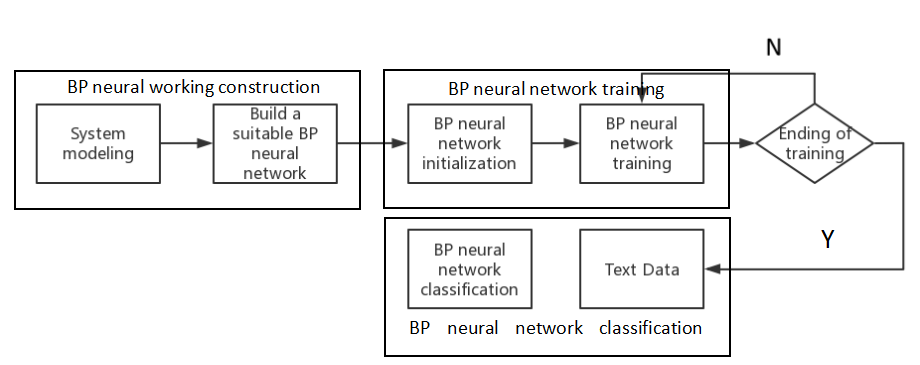
\includegraphics[scale=1.0]{ppp.png}
\caption{}
\label{fig:bp3}
\end{figure}


The construction of BP neural network determines the structure of the BP neural network according to the characteristics of the input and output data of the system. Since the input signal of the first-level indicator is 3-dimensional, there are 5 categories of national higher education health conditions to be evaluated, so the structure of the BP neural network is 3-5- 1. That is, the input layer has 3 nodes, the hidden layer has 5 nodes, and the output layer has 1 node.

When constructing the evaluation model of BP neural network, it is necessary to have a certain number of learning samples to establish an evaluation system. In order to minimize the evaluation error, we consider using the behavioral anchor quantification method to define different horizontal scales and construct a data set that meets the conditions as training samples.

Subsequently, the data from the United States and India were used to substitute the neural network for testing.

\subsubsection{Use particle swarm algorithm to improve BP neural network }

In the process of using the BP neural network to establish the evaluation model, there have been problems such as too long convergence time and large difference between the weight and threshold of each test. Therefore, we need to optimize and improve the BP neural network.

\textbf{Basic Principle of Particle Swarm Algorithm}

Some creatures in nature present group characteristics. For the convenience of research, people use a few simple rules to establish a movement model for group behavior. For example, Reynolds established the Bold model to simulate the flight of a flock of birds [39,40], and proposed three principles for individual flight in a flock:

\begin{enumerate}[\bfseries 1.]
    \item Fly away from the nearest companion.
    \item Flying towards the destination. 
    \item Move closer to the group center.

\end{enumerate}

Any individual in the group follows these three rules when flying. Inspired by the Bold model, in 1995, Kennedy and Eberhart simulated the foraging behavior of a flock of birds. They imagined a scenario where a group of birds was searching for food at random. There was only one piece of food in this area. At first, all the birds did not know that the food was there. There, but they knew which bird was the closest to the food, and the location that was the closest to the food, so each bird began to try to determine the flight direction of its search for food through these two locations. Particle swarm optimization algorithm is inspired from this model and is proposed to solve optimization problems. We can regard the foraging process of a flock of birds as an optimization problem, with each bird as a potential solution of the problem, and food as the optimal solution of the problem. Finding food for an individual is equivalent to finding the optimal solution for the optimization problem. All particles have a fitness value determined by the optimization function to measure their pros and cons. Each particle determines the direction and distance of their next flight based on the following information:

\begin{enumerate}[\bfseries 1.]
    \item Their current location. 
    \item Their own current speed.
    \item The distance between their current position and their historical best position.
    \item The distance between their current position and the historical best position of the entire group.
\end{enumerate}

In the particle swarm algorithm, the algorithm is initialized as a group of random particles (random solution), and then the optimal solution is found through iteration. In each iteration, the particle updates itself by tracking two "extreme values": the first is the optimal solution found by the particle itself, this is called the individual extreme value; the other extreme value is the maximum value currently found by the entire population. The optimal solution, this extreme value is the global extreme value, and then the particles search for the optimal position in the solution space.

The flow chart of the function extremum optimization algorithm based on the PSO algorithm is shown in the figure.


\begin{figure}[h!]
\centering
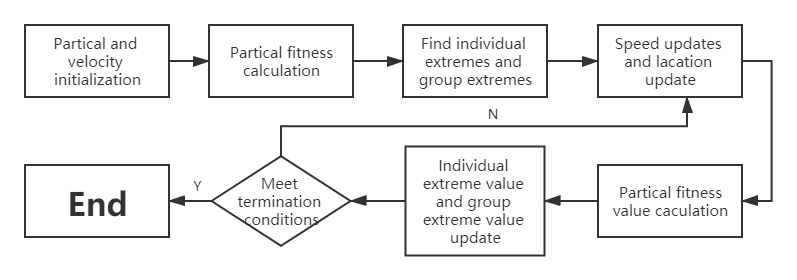
\includegraphics[scale=0.5]{biao3.png}
\caption{}
\label{fig:bp39}
\end{figure}


\subsubsection{The result of the problem}

According to the health evaluation model of the higher education system we have established, we can get the specific ratings of 5 countries as follows:

\begin{table}[hbt!]
\hspace{2.9cm}
\begin{tabular}{|l|l|l|l|l|l|}
\hline
        & United States & France & Japan & Brazil & India \\ \hline
Ratings & 5             & 3      & 3     & 2      & 1     \\ \hline
\end{tabular}
\end{table}






\subsection{Model 2: Sustainability Prediction Model }

\subsubsection{General idea}
The health evaluation model of the higher education system established above is based on current data, in order to evaluate the sustainability of the education system, we must establish a predictive model to predict the future higher education system at first, then bring the predicted value into the evaluation model to obtain the sustainability evaluation of the higher education system. 

\subsubsection{Grey prediction model}
Grey system theory is an emerging cross-discipline founded by the famous Chinese scholar Professor Deng Julong in 1982. It uses "small samples" and "poor information" uncertain systems with "part of the information is known and part of the unknown" as the research object. Mainly through the generation and development of part of the known information, and extracting valuable information, the correct understanding and exact description of the system operation law can be realized, and scientific predictions can be made accordingly.

The so-called gray system is a transitional system between the white system and the black box system. Its specific meaning is: if all the information of a certain system is known as a white system, all the information is unknown as a black box system, some information is known, and some information Unknown, then this system is a gray box system. Generally speaking, social systems, economic systems, and ecological systems are all gray systems.

Grey Prediction is based on Grey Model. Among many grey models, the single-sequence first-order linear differential equation model GM(1,1) model in grey system is the most commonly used. The following briefly introduces the GM (1,1) model.

Set the original data:

\begin{equation}\label{eq:heat2}\mathbf{x}^{(0)}=\left(x^{(0)}(1), x^{(0)}(2), \cdots, x^{(0)}(\mathrm{n})\right)\end{equation}

$n$ is the number of data.

If GM(1,1) is established based on the $x^{(0)}$  data column to realize the prediction function, the basic steps are as follows:

\begin{itemize}


\item  The original data is accumulated to weaken the volatility and randomness of the random sequence, and a new data sequence is obtained:

\begin{equation}\mathbf{x}^{(1)}=\left(x^{(1)}(1), x^{(1)}(2), \cdots, x^{(1)}(n)\right), \text { 其中 } x^{(1)}(\mathrm{t})=\sum_{k=1}^{t} x^{(0)}(t), t=0,1, \cdots, n\end{equation}

\item Establish a first-order linear differential equation for $x^{(1)}(t)$:

\begin{equation}\frac{d x^{(1)}(\mathrm{t})}{d t}+a x^{(1)}(\mathrm{t})=u\end{equation}

Among them, $a$, $u$ are undetermined coefficients, which are called development coefficient and gray effect, respectively, the effective interval of a is (-2, 2), and the matrix formed by a and u is  $\widehat{\mathbf{a}}=\left(\begin{array}{l}
a \\
u
\end{array}\right)$.

Only by asking for $a$, $u$, we can find $x^{(1)}(t)$, and then find the future predicted value of $x^{(0)}$.

\item Take the average of the accumulated data $x^{(1)}$ to get the column vector, and add a column of all 1 column vector to generate a matrix. Intercept the original sequence to obtain the column vector $Y$


\begin{equation}\label{eq:heat2}\mathbf{B}=\left[\begin{array}{cc}
-0.5\left(x^{(1)}(1)+x^{(1)}(2)\right) & , 1 \\
-0.5\left(x^{(1)}(2)+x^{(1)}(3)\right) & , 1 \\
\ldots & \\
-0.5\left(x^{(1)}(n-1)+x^{(1)}(n)\right) & , 1
\end{array}\right], \quad \mathbf{Y}=\left(x^{(0)}(1), x^{(0)}(2), \cdots, x^{(0)}(n)\right)^{T}\end{equation}

\item Use the least square method to solve the gray parameter. 

\hspace{5cm} $\widehat{\mathbf{a}}=\left(\begin{array}{l}
a \\
u
\end{array}\right)$\\

\hspace{4.3cm}
$\widehat{\mathbf{a}}=\left(\begin{array}{l}
a \\
u
\end{array}\right)=\left(\mathbf{B}^{T} \mathbf{B}\right)^{-1} \mathbf{B}^{T} \mathbf{Y}$

\item Bring  $\widehat{\mathbf{a}}=\left(\begin{array}{l}
a \\
u
\end{array}\right)$into $\frac{d x^{(1)}(\mathrm{t})}{d t}+a x^{(1)}(\mathrm{t})=u$, and solved:

\begin{equation}\hat{x}^{(1)}(t+1)=\left(x^{(0)}(1)-\frac{u}{a}\right) e^{-a t}+\frac{u}{a}\end{equation}

In order to distinguish it from the original sequence $x^{(1)}(t)$, it is recorded as $\hat{x}^{(1)}(t+1)$ .

\item  Discrete function expressions  $\hat{x}^{(1)}(t+1)$ and $\hat{x}^{(1)}(t)$ , And subtract the two to restore the original sequence of $x^{(0)}$ , The approximate data sequence  $\hat{x}^{(0)}(t+1)$ is as follows:

\end{itemize}
\begin{equation}\bar{x}^{(0)}(t+1)=\bar{x}^{(1)}(t+1)-\tilde{x}^{(1)}(t)\end{equation}

According to the formula, we can get the forecast value of 5 countries in the third year:

\begin{table}[hbt!]
\hspace{3.7cm}
\begin{tabular}{|l|l|l|l|l|l|}
\hline

   & United States & France & Japan & Brazil & India \\ \hline
A1 & 1.61          & 0.45   & 0.46  & 1.32   & -0.56 \\ \hline
A2 & 1.45          & -0.12  & 0.87  & -1.89  & 0.47  \\ \hline
A3 & -1.77         & 0.72   & 0.69  & 2.21   & 1.32  \\ \hline
\end{tabular}
\end{table}







\subsubsection{Higher education sustainability results}

Bring the predicted results into the previous national higher education health evaluation model, and the result obtained is the sustainable evaluation of national higher education. The specific ratings of the six countries are:

\begin{table}[hbt!]
\hspace{3.3cm}
\begin{tabular}{|l|l|l|l|l|l|}
\hline
        & United States & France & Japan & Brazil & India \\ \hline
Ratings & 5             & 4      & 3     & 2      & 1     \\ \hline
\end{tabular}
\end{table}





\subsection{Japan's Higher Education Reform Plan}

\subsubsection{Analysis of current situation in Japan}

According to the two models in the previous article, Japan’s higher education health evaluation is level 3 and sustainability evaluation is level 4. Japan has the potential to build a more sound and perfect education system in the future. The Japanese government attaches great importance to higher education, provides a large amount of capital investment every year, and has achieved remarkable results. As an emerging country in education, Japan’s Nobel Prize and Fields Prize surpassed most countries in the world in a short period of time, which is sufficient proof of the effectiveness of Japan’s educational reform. However, compared with the United States, there is still a certain gap in the level of higher education in Japan. The key factor restricting its development is the low enrollment rate. Compared with Australia's over 100\% enrollment rate, Japan’s enrollment rate is in urgent need of increasing.

\subsubsection{Targeted policies and implementation timetable}

In response to Japan’s low enrollment rate, we have proposed a policy that includes increasing the number of universities, expanding the number of university enrollments, and attracting international students. By implementing this policy, the enrollment rate in Japan is expected to increase by more than 6\% per year. Substituting data into our model can be obtained. After three years, the health and sustainability of the Japanese higher education system can reach level 4. If it lasts longer, Japan is likely to reach a level similar to that of the United States.

\subsubsection{ Difficulties and challenges faced by change}

The pertinent plan we put forward is only to modify and improve the data, but in reality, in addition to considering the impact from the theory, we must also consider the constraints brought about by the actual situation.

\begin{itemize}
\item The population aging in Japanese society is becoming more and more serious. The proportion of 65-year-olds is close to 30\%, and the new population is decreasing year by year. This means that the goal of increasing enrollment is more difficult to implement

\item For the majority of international students, Japan is not as selective as English-speaking countries due to the limited practicality of Japanese. It is difficult for the Japanese government to overcome this problem to increase Japan’s attractiveness for studying abroad

\item The Japanese government's cabinet changes frequently, and it is difficult to implement the unified policy for a long time.

\item Due to the impact of the new crown epidemic this year, the Japanese government must focus its energy on prevention and control and fighting the epidemic, and its investment in education will inevitably decrease


\end{itemize}




\section{Evaluation of the models}

\subsection{Strengths}

\begin{enumerate}[\bfseries 1.]

\item Particle swarm optimization (PSO) is a new swarm intelligence algorithm which has many advantages in optimizing neural networks:

\begin{itemize}
    \item  Particle swarm optimization (PSO) is based directly on the fitness function value of the change of the objective function.
    \item Particle swarm optimization (PSO) is a random optimization method, which starts from the population of multiple points. It has strong global search ability, can find the global optimal value with a large probability, and can effectively avoid BP neural network falling into local minimum value.
    \item The whole process of searching and updating PSO is the process of following the current optimal solution, which is one-way information flow. In most cases, all particles may converge to the global optimal solution faster.
    \item Particle swarm optimization can not only optimize the connection weights and thresholds of neural networks, but also optimize the topology of neural networks and effectively improve the overall search performance of neural networks.

\end{itemize}

\item This paper starts from many angles in model construction and data selection, and selects different levels of countries to analyze, which is objective and representative.

\item The model constructed in this paper, on the basis of consulting a large number of relevant materials, it absorbs their advantages, and has its own unique innovation and has certain reference value.

\end{enumerate}

\subsection{Weaknesses}

\begin{enumerate}[\bfseries 1.]

\item Although BP algorithm has nonlinear ability and strong fault-tolerant ability, it also has the following disadvantages because the algorithm is essentially gradient descent method:


\begin{itemize}
    \item The convergence speed of learning process is slow BP the objective function of algorithm optimization is very complex, the error surface has flat region, and the convergence speed is slow due to the small change of error gradient.
    \item Network training is easy to fall into local extremum BP network training is from a certain starting point of the slope gradually reached the minimum error. The error function of BP neural network is a surface with multipolar multidimensional space, but the BP algorithm only follows the direction of error function descent, so in its training process, the network often falls into local minimum point.
    \item The structure of the network is difficult to determine the structural parameters of the network, especially the number of hidden layers and the number of hidden layer neurons, which lack theoretical guidance and can only be selected according to experience or experiment.
    \item The generalization ability of the network is difficult to guarantee. In general, the generalization ability of the network increases with the improvement of the training ability, but the trend has a limit.
 \end{itemize}

\item The present is a special period of global epidemic, the epidemic will have incalculable changes in higher education. Due to our lack of data on the impact of the epidemic on higher education, our model has some limitations

\item For a very small number of countries, we do not have access to data and therefore do not allow for data verification in these particular countries

\end{enumerate}
\section{Improvement and Extension of Models}

\subsection{Modelling Improvements:}
    Due to the defects of BP network itself, the further development and application of BP network have been greatly affected.In the past ten years, many researchers have done a lot of work to improve the performance of the algorithm and proposed many improved methods.It can be divided into the following aspects: 
 \begin{itemize}
    \item Add momentum term.The standard BP algorithm is actually a simple steepest descent static optimization algorithm,in the process of revising the weight,first,the weight adjustment at time k is only corrected according to the negative gradient direction at time k,without considering the direction of gradient change before that(the experience accumulated in network training). As a result, the training process oscillates and the convergence speed is slow. For this reason, many scholars proposed improved methods of momentum term.This method is the weight adjustment amount. On the basis of the current weight amount,scholars add an amount proportional to the previous weight adjustment amount,the added momentum term is equivalent to the damping term.It reduces the oscillation tendency of the learning process, thereby improving convergence.
    \item Improve learning rate.In the standard BP algorithm, the learning rate generally selected in the network learning process is always a constant,in actual training,it is hoped to increase the learning rate in a flat area so that the training can escape the area faster;In some steep areas,it is hoped to reduce the learning rate to avoid network training oscillations or even divergence,so in order to get a better training effect, the general method is to adjust the learning rate adaptively.
    \item Improve the activation function.The standard BP algorithm uses the Sigmoid function as the activation function. The derivative of this function is simple and similar to the true reflection of biological neurons.
    
    However, when the neuron's net input is too large or too small, the output will enter the saturation region, resulting in non-convergence.The current improved algorithms include: using a piecewise function as the activation function and introducing a steepness factor into the activation function.
    
    \item Improve and optimize algorithm.The standard BP algorithm uses gradient descent,which makes the training easy to fall into a local minimum and makes the convergence speed slow.The current improved algorithms include: a second-order learning algorithm based on the Block Hessian matrix,which effectively avoids the shortcomings of the standard BP algorithm.
    \item Optimize the initial weight standard of the network.The initial weight of the BP algorithm is a set of random numbers, and the initial weight of the network is not well selected, which makes it is easy to fall into a local minimum.Use Cauchy's inequality and linear algebra method to optimize the initial weights which,effectively accelerate the convergence speed.
    \item Combine with intelligent algorithms.At present,commonly used evolutionary intelligent algorithms include genetic algorithm,Ant colony optimization algorithms, artificial immune algorithm, particle swarm optimization algorithm.Intelligent algorithms have good global optimization capabilities, while standard BP algorithms have good local optimization capabilities, so the two can be combined.

\end{itemize}
\subsection{Extension of the Model}
The health evaluation model and the sustainable evaluation model established in this paper can not only be evaluated in higher education, but also in various industries, such as politics, economy, military, agriculture and so on[10]The results are more accurate and objective and have more reference value.
% 以下为信件/备忘录部分,不需要可自行去掉
% 如有需要可将整个 letter 环境移动到文章开头或中间
% 请在第二个花括号内填写标题,如「信件」(Letter)或「备忘录」(Memorandum)

\vfill

\begin{thebibliography}{99}
\bibitem{1} Liu Yang et al. "Thermal error prediction of motorized spindle for five-axis machining center based on analytical modeling and BP neural network". 35.1(2021):281-292.
\bibitem{2} A. S. Elons, Dalia Ahmed Magdi, M. Y. Elgendy, "A proposed model for predicting the drilling path based on hybrid Pso-Bp neural network", SAI Computing Conference (SAI) 2016, pp. 148-155, 2016.
\bibitem{3} Junhe Zhou, Jianping Chen, Xinwan Li, Guiling Wu, Yiping Wang, Wenning Jiang, "Robust compact and flexible neural model for a fiber Raman amplifier", Lightwave Technology Journal of, vol. 24, no. 6, pp. 2362-2367, 2006.

\bibitem{4} M. S. Al-Duais, A. R Yaakub, N. Yusoff, "Dynamic training rate for backpropagation learning algorithm", Communications (MICC) 2013 IEEE Malaysia International Conference on, pp. 277-282, 2013.


\bibitem{5} A. Goedtel, I. Nunes da Silva, P.J.A. Semi, "An alternative approach to solve convergence problems in the backpropagation algorithm", Neural Networks 2004. Proceedings. 2004 IEEE International Joint Conference on, vol. 2, pp. 1021-1026 vol.2, 2004.



\bibitem{6} "Notice to IEEE Xplore subscribers", Applied Robotics for the Power Industry (CARPI) 2012 2nd International Conference on, 2012.

\bibitem{7} Xuechun Wang, Wendong Chen, Yuan Ji, Feng Ran, "Gesture recognition based on parallel hardware neural network implemented with stochastic logics", Audio Language and Image Processing (ICALIP) 2016 International Conference on, pp. 534-539, 2016.



\end{thebibliography}


% 以下为附录内容
% 如您的论文中不需要附录,请自行删除
\begin{subappendices}  % 附录环境


\section{Appendix A: Program Codes}
Here are some core codes we used in our research.

% 代码环境示例三则
% 如您的论文不需要展示代码,请删除
% 更多用法,请参考 listings 宏包文档

% Python 代码示例
\begin{lstlisting}[language=Python, name={my1.py}]
# Python
import numpy as np
from pyswarm import pso

# Define the objective (to be minimize)
def weight(x, *args):
    H, d, t = x
    B, rho, E, P = args
    return rho*2*np.pi*d*t*np.sqrt((B/2)**2 + H**2)

# Setup the constraint functions
def yield_stress(x, *args):
    H, d, t = x
    B, rho, E, P = args
    return (P*np.sqrt((B/2)**2 + H**2))/(2*t*np.pi*d*H)

def buckling_stress(x, *args):
    H, d, t = x
    B, rho, E, P = args
    return (np.pi**2*E*(d**2 + t**2))/(8*((B/2)**2 + H**2))

def deflection(x, *args):
    H, d, t = x
    B, rho, E, P = args
    return (P*np.sqrt((B/2)**2 + H**2)**3)/(2*t*np.pi*d*H**2*E)

def constraints(x, *args):
    strs = yield_stress(x, *args)
    buck = buckling_stress(x, *args)
    defl = deflection(x, *args)
    return [100 - strs, buck - strs, 0.25 - defl]


\end{lstlisting}

\begin{lstlisting}[language=Python, name={my2.py}]
# Define the other parameters
B = 60  # inches
rho = 0.3  # lb/in^3
E = 30000  # kpsi (1000-psi)
P = 66  # kip (1000-lbs, force)
args = (B, rho, E, P)

# Define the lower and upper bounds for H, d, t, respectively
lb = [10, 1, 0.01]
ub = [30, 3, 0.25]

xopt, fopt = pso(weight, lb, ub, f_ieqcons=constraints, args=args)

# The optimal input values are approximately
#     xopt = [29, 2.4, 0.06]
# with function values approximately
#     weight          = 12 lbs
#     yield stress    = 100 kpsi (binding constraint)
#     buckling stress = 150 kpsi
#     deflection      = 0.2 in


# Setup the constraint functions
def yield_stress(x, *args):
    H, d, t = x
    B, rho, E, P = args
    strs = (P*np.sqrt((B/2)**2 + H**2))/(2*t*np.pi*d*H)
    return 100 - strs

def buckling_stress(x, *args):
    H, d, t = x
    B, rho, E, P = args
    buck = (np.pi**2*E*(d**2 + t**2))/(8*((B/2)**2 + H**2))
    strs = yield_stress(x, *args)
    return buck - strs

def deflection(x, *args):
    H, d, t = x
    B, rho, E, P = args
    defl = (P*np.sqrt((B/2)**2 + H**2)**3)/(2*t*np.pi*d*H**2*E)
    return 0.25 - defl

...

cons = [yield_stress, buckling_stress, deflection]

...

xopt, fopt = pso(weight, lb, ub, ieqcons=cons, args=args)



\end{lstlisting}


\end{subappendices}  % 附录内容结束

\end{document}  % 结束
